\section{Auswertung}
\subsection{Längenmessung}
Es werden die Längen von vier verschiedenen Koaxialkabeln bestimmt.
Dazu wird der zeitliche Abstand zwischen einlaufendem und 
reflektierten Signal auf einem Oszilloskop betrachtet.\\
In den Abbildungenn~\ref{fig:laenge_rot},~\ref{fig:laenge_schwarz},
~\ref{fig:laenge_gruen} und ~\ref{fig:laenge_trommel} sind die 
verwendeten Bilder zu sehen. Die Zeitmessung wird an den dort 
rot eingezeichneten Markierungen vorgenommen.\\
In Tabelle~\ref{tab:laengenmessung} sind die abgelesenen Zeitabstände 
eingetragen. Ebenso in dieser Tabelle sind die mit den Zeitabständen 
mit Hilfe von Formel~\eqref{eq:laengenrechnung} errechneten 
Längen der Kabel eingetragen. Dabei bezeichnet c die Lichtgeschwindigkeit. 
Der Wert \SI{2.25}{} gibt den Dielektrizitätswert der Kabel an.
%
\begin{equation}
L = \frac{c\cdot\Delta t}{2\cdot\sqrt{2,25}}
\label{eq:laengenrechnung}
\end{equation}
%
\begin{table}[h]
  \centering
  \begin{tabular}{SS|S}
    \toprule
{Kabel}&{Signalabstand }$\Delta${t/}\si{\nano\second}&{Kabellänge/}\si{\metre}\\
\midrule
{Rot}&18&1.8\\
{Schwarz}&116&11.6\\
{Grün}&85&8.5\\
{Trommel}&822&82.1\\
\bottomrule
  \end{tabular}
  \caption{LÄNGENMSSSUNG.}
  \label{tab:laengenmessung}
\end{table}
%
\begin{figure}
  \centering

  \begin{subfigure}{0.4\textwidth}
    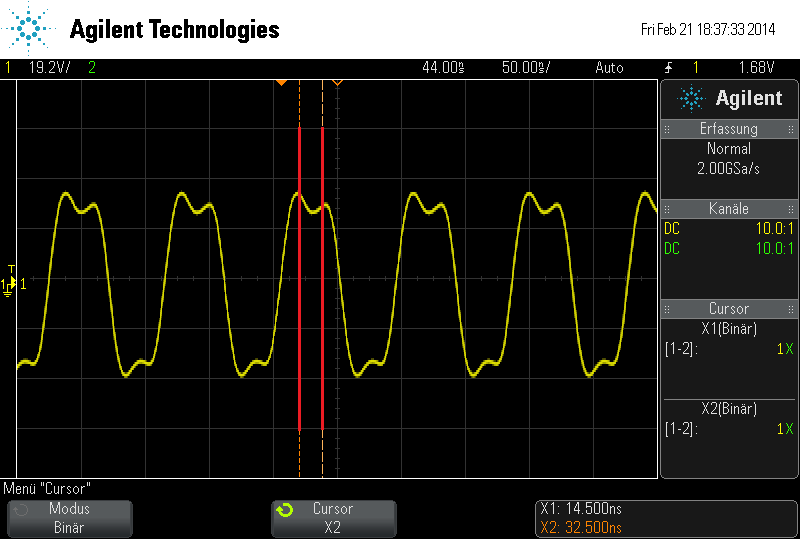
\includegraphics[width=\textwidth]{laenge_rot.png}
    \caption{rotes Kabel}
    \label{fig:laenge_rot}
  \end{subfigure}
  \quad
  \begin{subfigure}{0.4\textwidth}
    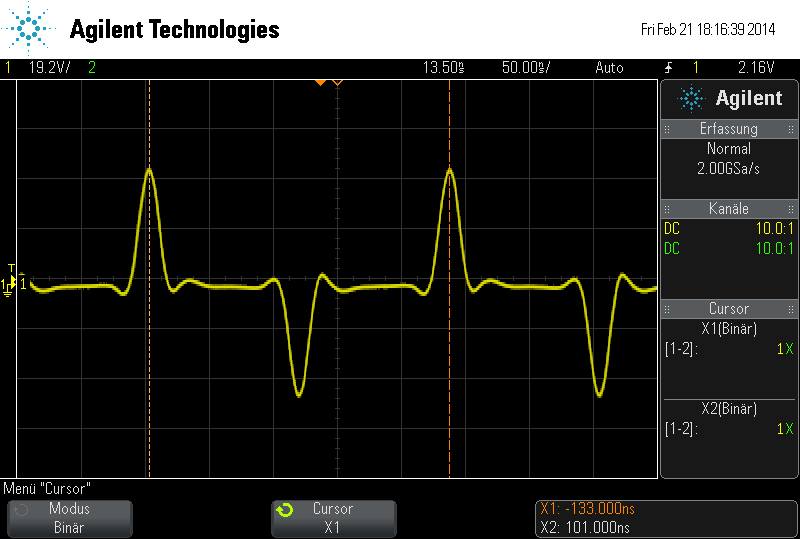
\includegraphics[width=\textwidth]{laenge_schwarz.png}
    \caption{schwarzes Kabel}
    \label{fig:laenge_schwarz}
  \end{subfigure}

  \begin{subfigure}{0.4\textwidth}
    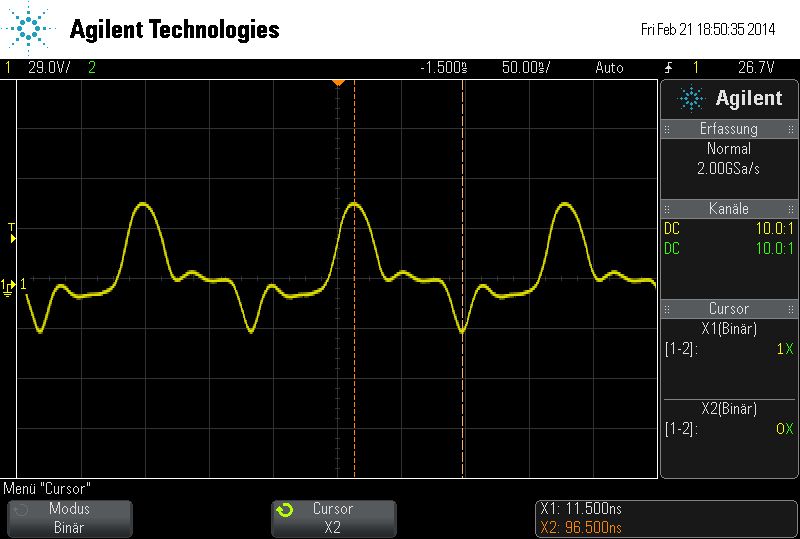
\includegraphics[width=\textwidth]{laenge_gruen.png}
    \caption{grünes Kabel}
    \label{fig:laenge_gruen}  
  \end{subfigure}
  \quad
  \begin{subfigure}{0.4\textwidth}
    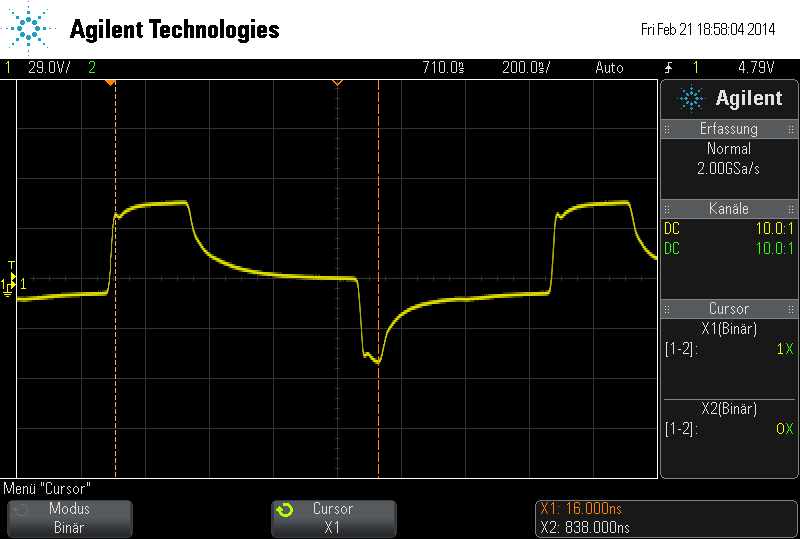
\includegraphics[width=\textwidth]{laenge_trommel.png}
    \caption{Kabeltrommel}
    \label{fig:laenge_trommel}
  \end{subfigure}

  \caption{Längenmessung}
\end{figure}
%
\FloatBarrier
%
\subsection{Belagsmessung}
%
Die mit einem LRC-Messgerät bestimmten Induktivitäten ${L}_\text{g}$, 
Widerstände ${R}_\text{g}$ und Kapazitäten ${C}_\text{g}$ bei verschiedenen 
Frequenzen f sind für das rote Kabel in 
Tabelle~\ref{tab:RLC_rot}, für das schwarze Kabel in 
Tabelle~\ref{tab:RLC_schwarz}, und für die Kabeltrommel in 
Tabelle~\ref{tab:RLC_trommel} aufgeführt.
Ebenfalls in diesen Tabellen sind sowohl die mit
Formel~\eqref{eq:belagsformel} berechneten Querleitwerte ${G}_\text{g}$ 
der jeweiligen Kabel aufgeführt, als auch die durch die Längen der 
Kabel errechneten Beläge R, L, C und G.
%
\begin{table}[h]
  \centering
  \sisetup {
	per-mode = fraction
  }
  \begin{tabular}{SSSSSSSSS}
    \toprule
{f /}\si{\kilo\hertz}&
${R}_\text{g}${/}\si{\ohm}&{R/}\si{\ohm\per\metre}&
${L}_\text{g}${/}\si{\micro\henry}&{L/}\si{\micro\henry\per\metre}&
${C}_\text{g}${/}\si{\pico\farad}&{C/}\si{\pico\farad\per\metre}&
${G}_\text{g}${/}\si{\micro\siemens}&{G/}\si{\micro\siemens\per\metre}\\
\midrule
0.05&2.47&1.37&4.5&2.50&138.8&77.2&76.2&42.4\\
0.10&2.48&1.38&4.5&2.50&138.8&77.2&76.5&42.5\\
0.20&2.48&1.38&4.4&2.45&138.8&77.2&78.2&43.5\\
0.30&2.48&1.38&4.6&2.56&138.8&77.2&74.8&41.6\\
0.50&2.48&1.38&4.5&2.50&138.8&77.2&76.5&42.5\\
0.80&2.48&1.38&4.3&2.40&138.8&77.2&80.0&44.5\\
1.00&2.49&1.38&4.2&2.33&138.8&77.2&82.3&45.7\\
1.50&2.49&1.38&4.1&2.28&138.8&77.2&84.3&46.9\\
2.00&2.50&1.39&4.0&2.22&138.7&77.1&86.7&48.2\\
3.00&2.51&1.40&3.8&2.10&138.7&77.1&92.3&51.3\\
5.00&2.53&1.41&3.4&1.89&138.6&77.1&103.1&57.3\\
7.00&2.55&1.42&3.2&1.78&138.6&77.1&110.4&61.4\\
10.00&2.56&1.42&3.0&1.67&138.6&77.1&118.3&65.8\\
14.00&2.58&1.43&2.8&1.56&138.5&77.0&127.6&70.9\\
18.00&2.59&1.44&2.8&1.56&138.5&77.0&128.1&71.2\\
20.00&2.60&1.45&2.7&1.50&138.5&77.0&133.4&74.1\\
100.00&2.60&1.45&2.6&1.45&138.6&77.1&138.6&77.1\\
\bottomrule
  \end{tabular}
  \caption{RLCROT}
  \label{tab:RLC_rot}
\end{table}
%
\begin{table}[h]
  \centering
  \sisetup {
	per-mode = fraction
  }
  \begin{tabular}{SSSSSSSSS}
    \toprule
{f /}\si{\kilo\hertz}&
${R}_\text{g}${/}\si{\ohm}&{R/}\si{\ohm\per\metre}&
${L}_\text{g}${/}\si{\micro\henry}&{L/}\si{\micro\henry\per\metre}&
${C}_\text{g}${/}\si{\pico\farad}&{C/}\si{\pico\farad\per\metre}&
${G}_\text{g}${/}\si{\micro\siemens}&{G/}\si{\micro\siemens\per\metre}\\
\midrule
0.05&2.41&0.21&8.8&0.76&1100&94.9&301.3&26.0\\
0.10&2.41&0.21&7.3&0.63&988&85.2&326.2&28.1\\
0.20&2.41&0.21&7.1&0.61&988&85.2&335.4&29.0\\
0.30&2.41&0.21&7.0&0.60&988&85.2&340.2&29.3\\
0.50&2.41&0.21&7.2&0.62&988&85.2&330.7&29.0\\
0.80&2.41&0.21&7.0&0.60&988&85.2&340.2&29.3\\
1.00&2.41&0.21&6.9&0.59&988&85.2&345.1&29.8\\
1.50&2.41&0.21&6.8&0.59&988&85.2&350.2&30.2\\
2.00&2.41&0.21&6.7&0.58&988&85.2&355.4&30.7\\
3.00&2.42&0.21&6.4&0.55&988&85.2&373.6&32.2\\
5.00&2.43&0.21&6.0&0.52&988&85.2&400.1&34.5\\
7.00&2.44&0.21&5.8&0.50&988&85.2&415.6&35.9\\
10.00&2.45&0.21&5.6&0.48&988&85.2&432.3&37.3\\
14.00&2.45&0.21&5.5&0.47&988&85.2&440.1&38.0\\
18.00&2.46&0.21&5.4&0.47&988&85.2&450.1&38.8\\
20.00&2.46&0.21&5.4&0.47&988&85.2&450.1&38.8\\
100.00&2.60&0.22&5.2&0.45&990&85.4&495.0&42.7\\
\bottomrule
  \end{tabular}
  \caption{RLCSCHWARZ}
  \label{tab:RLC_schwarz}
\end{table}
%
\begin{table}[h]
  \centering
  \sisetup {
	per-mode = fraction
  }
  \begin{tabular}{SSSSSSSSS}
    \toprule
{f /}\si{\kilo\hertz}&
${R}_\text{g}${/}\si{\ohm}&{R/}\si{\ohm\per\metre}&
${L}_\text{g}${/}\si{\micro\henry}&{L/}\si{\micro\henry\per\metre}&
${C}_\text{g}${/}\si{\nano\farad}&{C/}\si{\nano\farad\per\metre}&
${G}_\text{g}${/}\si{\milli\siemens}&{G/}\si{\milli\siemens\per\metre}\\
\midrule
0.05&4.44&0.05&22.8&0.27&8.39&0.10&1.69&0.02\\
0.10&4.43&0.05&22.8&0.27&8.50&0.10&1.71&0.02\\
0.20&4.43&0.05&25.0&0.30&8.50&0.10&1.51&0.02\\
0.30&4.42&0.05&25.6&0.31&8.50&0.10&1.47&0.02\\
0.50&4.42&0.05&26.3&0.32&8.50&0.10&1.43&0.02\\
0.80&4.41&0.05&26.1&0.32&8.50&0.10&1.44&0.02\\
1.00&4.41&0.05&26.0&0.32&8.50&0.10&1.44&0.02\\
1.50&4.42&0.05&25.9&0.32&8.50&0.10&1.45&0.02\\
2.00&4.42&0.05&25.9&0.32&8.50&0.10&1.45&0.02\\
3.00&4.41&0.05&25.9&0.32&8.50&0.10&1.45&0.02\\
5.00&4.41&0.05&25.9&0.32&8.50&0.10&1.45&0.02\\
7.00&4.42&0.05&25.9&0.32&8.50&0.10&1.45&0.02\\
10.00&4.42&0.05&25.9&0.32&8.50&0.10&1.45&0.02\\
14.00&4.43&0.05&25.9&0.32&8.50&0.10&1.45&0.02\\
18.00&4.44&0.05&25.9&0.32&8.51&0.10&1.46&0.02\\
20.00&4.45&0.05&25.9&0.32&8.51&0.10&1.46&0.02\\
100.00&5.29&0.06&26.4&0.32&8.75&0.11&1.75&0.20\\
\bottomrule
  \end{tabular}
  \caption{RLCTROMMEL}
  \label{tab:RLC_trommel}
\end{table}
%
Einen Plot der Leitungsbelagswerte in Abhängigkeit von der Frequenz 
für die verschiedenen Kabel ist in Plot~\ref{fig:belaege} zu sehen.
%
\begin{figure}[]
\centering
\includegraphics[width=1\textwidth]{4er.pdf}
\caption{4ER}
\label{fig:belaege}
\end{figure}
%
\FloatBarrier
%
\subsection{Dämpfungsbestimmung}
%
Um die Dämpfungskonstante $\alpha$ der Kabeltrommen zu bestimmen, 
wird die Fouriertransformation eines Rechtecksignals betrachtet. Die 
für ein sehr kurzes Kabel und die Kabeltrommen erhaltenen FFT-Bilder 
sind in den Bildern~\ref{fig:daempfung_kurz} 
und~\ref{fig:daempfung_lang} zu sehen.\\
In Tabelle~\ref{tab:daempfung} sind die abgelesenen Amplituden der 
erkennbaren Maxima eingetragen, sowie das Verhältnis von den 
ungedämpften zu den gedämpften Amplituden, welches die 
Dämpfung angibt. Teilt man diese durch die Länge des verwendeten 
Kabels, so ergibt sich die gesuchte Dämpfungskonstante $\alpha$.
%
\begin{figure}[]
\centering
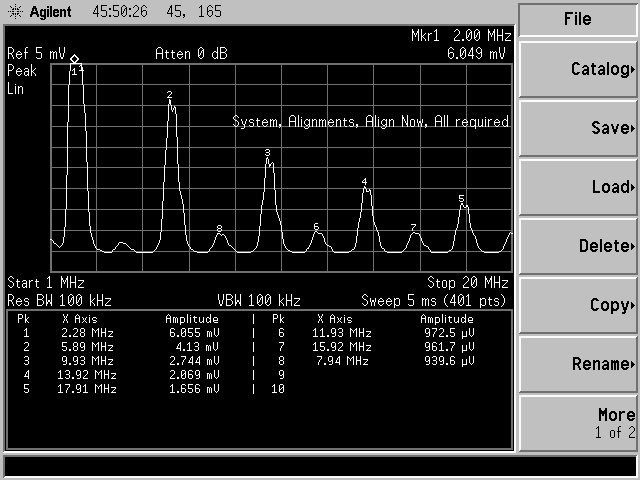
\includegraphics[width=0.8\textwidth]{daempfung_kurz.png}
\caption{KURZ}
\label{fig:daempfung_kurz}
\end{figure}
%
\begin{figure}[]
\centering
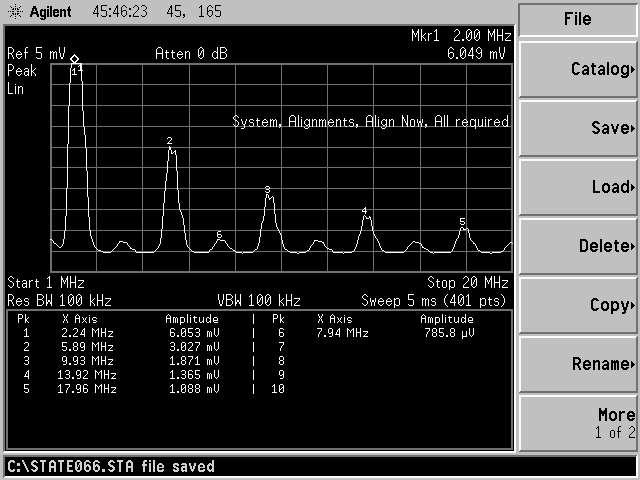
\includegraphics[width=0.8\textwidth]{daempfung_lang.png}
\caption{LANG}
\label{fig:daempfung_lang}
\end{figure}
%
\begin{table}[h]
  \centering
  \begin{tabular}{SSSSS}
    \toprule
{Nr.}&${U}_\text{ungedämpft}${/}\si{\milli\volt}&${U}_\text{gedämpft}{ /}\si{\milli\volt}$&
$\frac{{U}_\text{ungedämpft}}{{U}_\text{gedämpft}}$&
$\alpha${ /}\si{\per\metre}\\
\midrule
1&6.005&6.053&0.992&0.012\\
2&4.130&3.027&1.364&0.017\\
3&2.744&1.871&1.467&0.018\\
4&2.069&1.365&1.516&0.018\\
5&1.656&1.088&1.522&0.019\\
\midrule
\multicolumn{3}{c}{Mittelwerte: }&\SI{1.372(89)}{}&\SI{0.017(1)}{}\\
\bottomrule
  \end{tabular}
  \caption{DÄMPFUNG}
  \label{tab:daempfung}
\end{table}
%
\subsection{Mehrfacheflexion}
%
Nun wird das Signal untersucht, welches entsteht, wenn zwei 
Kabel mit unterschiedlichen Ohmschen Widerständen in Reihe geschaltet 
werden. Das erste Kabel besitzt einen Ohmschen Widerstand von 
\SI{50}{\ohm}, das zweite \SI{75}{\ohm}.\\
Abbildung~\ref{fig:impulsfahrplan} zeigt den dazugehörigen 
Impulsfahrplan, Abbildung~\ref{fig:mehrfachreflex} das mit einem 
Oszilloskopen aufgenommene Bild.\\
Tabelle~\ref{tab:mehrfachreflex} enthält die gemessenen Sprunghöhen 
in der Spannung und die daraus berechneten Reflexionskoeffizienten. 
Dabei bezeichnet $\Gamma_{50}$ den Reflexionsfaktor am Ende des 
\SI{50}{\ohm} Kabels und $\Gamma_{75}$ entsprechend den 
Reflexionsfaktor am Ende des \SI{75}{\ohm} Kabels, also dem offenen 
Ende.\\
Wie bereits in der Durchführung erwähnt, wird der Sprung zwischen 
Sprung Zwei und Drei nicht gemessen, da vernachlässigbar.\\
Dadurch ergeben sich durch einfache Überlegungen die in 
den Formeln~\eqref{eq:sprung1}, ~\eqref{eq:sprung2} 
und ~\eqref{eq:sprung3} angegebenen Relationen.
%
\begin{equation}
\text{Sprung1} = U_0
\end{equation}
%
\begin{equation}
\frac{\text{Sprung2}}{\text{Sprung1}} = \Gamma_{50}
\end{equation}
%
\begin{equation}
\frac{\text{Sprung3}}{\text{Sprung1}\cdot\left(1 - \Gamma_{50}\right)} = \Gamma_{75}
\end{equation}
%
\begin{figure}[]
\centering
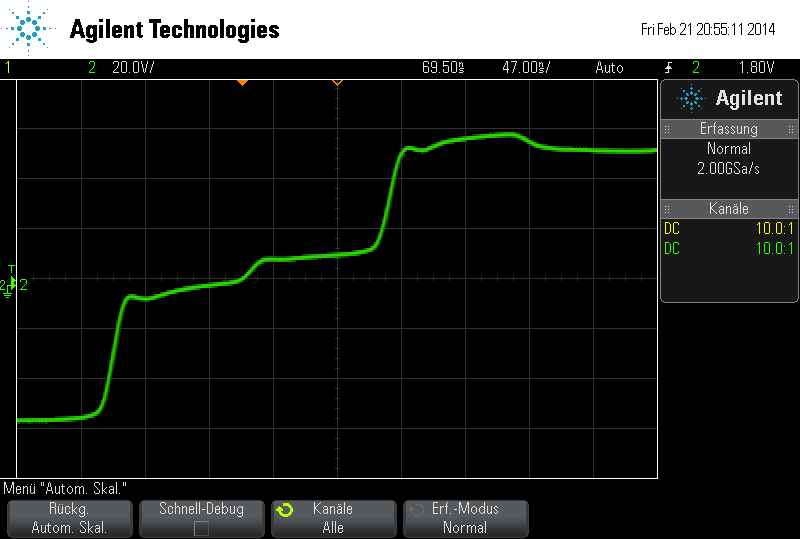
\includegraphics[width=0.8\textwidth]{reflex.png}
\caption{MEHRFACHREFLEX}
\label{fig:mehrfachreflex}
\end{figure}
%
\begin{table}[h]
  \centering
  \begin{tabular}{SS|SS}
    \toprule
{Sprung Nr.}&{Sprunghöhe /}\si{\volt}&
{Größe}&{Wert}\\
\midrule
1&50&{$U_0$}&50\si{\volt}\\
2&8.2&{$\Gamma_{50}$}&0.16\\
3&44.5&{$\Gamma_{75}$}&1.06\\
\bottomrule
  \end{tabular}
  \caption{MEHRFACHREFLEX}
  \label{tab:mehrfachreflex}
\end{table}
%
\FloatBarrier
%
\subsection{Verschiedene Abschlusswiderstände}
%
In diesem Abschnitt werden die erhaltenen Signalspannungen 
für verschiedene unbekannte Abschlusswiderstände mit den im 
Theorieteil berechneten Signalspannungen verglichen, um so 
auf die Art des Abschlusses und die dazugehörige Zeitkonstante 
zu schliessen.\\
Die Paragraphen sind nach den verwendeten Kästen und Buchsen 
benannt.\\\\

\paragraph{Kasten 2 Buchse 3}
Der sich bei diesem Abschluss ergebende Signalverlauf ist in 
Bild~\ref{fig:k2b3} zu sehen. Der Fit mit der 
Funktion~\eqref{eq:ind_ohm_reflex}, welche zu dem in Reihe geschalteten 
ohmschen Widerstand und einer Induktivität gehört, liefert das 
beste Ergebnis. Das Ergebnis dieses Fits ist in 
Formel~\eqref{eq:fit_k2b3} wiedergegeben.\\
Daraus ergibt sich die Zeitkonstante in~\eqref{eq:zeit_k2b3}.\\
Plot~\ref{fig:fit_k2b3} zeigt die gefittete Kurve durch Punkte, die 
am Oszilloskop aus dem Signalverlauf abgelesen wurden.\\
%
\begin{figure}[]
\centering
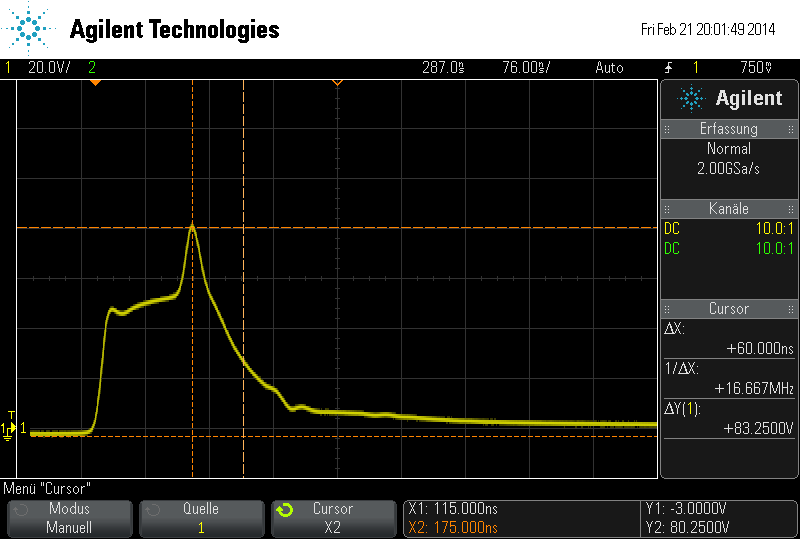
\includegraphics[width=0.8\textwidth]{k2b3.png}
\caption{K2B3OSZI}
\label{fig:k2b3}
\end{figure}
%
\begin{equation}
U(t) = \SI{41.625}{\volt}\cdot\left(2 - 
1.87\left(1-\exp{\left(\frac{-t}{\SI{4.89}{\second}}\right)}
\right)\right)
\end{equation}
%
\begin{equation}
\tau = \frac{L}{Z_0 + R} = \SI{1}{\second}
\end{equation}
%
3 versch. Abschlusswiderstände 
3 Bilder
Tabelle mit Messwerten
Funktion aus Theorie
Fit ( Bilder + Parameter => Zeitkonst.)
%
